
\chapter{پیشنهاد دهنده کالا وخدمات }
\section{مقدمه}

 در سال های اخیر خرید کالا ویا استفاده از خدمات آنلاین افزایش یافته است . 
سیستم‌های پیشنهاد ‌کننده ابزارهای مهمی برای مصرف کنندگان برای شناسایی کالاها وخدمات مورد علاقه خود و نیز برای کسب‌وکارها برای بهبود محصولات و خدمات خود هستند.
انتخاب و رزرو هتل 
 \cite{abbasi2019grouping}
یا رستوران
\cite{asani2021restaurant}
به صورت آنلاین هم شاهد رشد پررونقی بوده است و نقش این پیشنهاد دهنده های هوشمند در این رشد موثر بوده است ؛ در ادامه به بررسی یکی از این سیستم های پیشنهاد دهنده هتل به عنوان عامل هوشمند می پردازیم . 
\begin{figure}[h]
	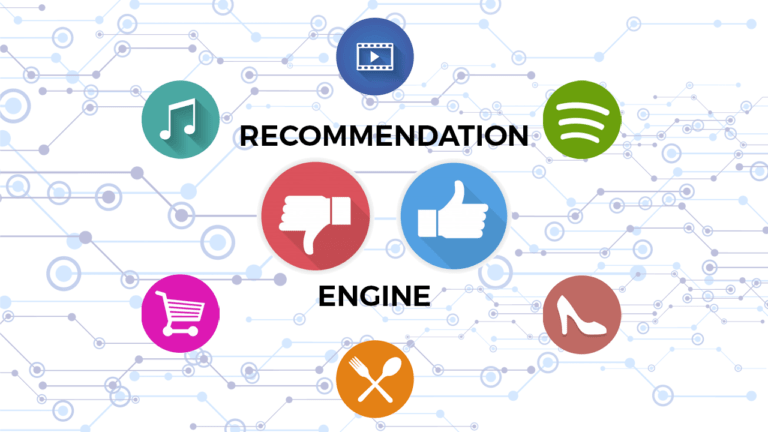
\includegraphics[scale=0.5]{reccomendation_sys}
	\centering
	\caption{موتورهای پیشنهاد دهنده کالا و خدمات}
	\cite{Naveennomidl}
	\label{rec_sys:fig1}
\end{figure} 
\section{طرح مسئله}
سیستم‌های توصیه‌کننده به عنوان یکی از عوامل موثر در رونق برخی از پلتفرم های آنلاین به شمار می روند . این سیستم ها براساس داده های رضایتمندی مشتریان ، میزان فروش کالا و خدمات وسلیقه و علاقه مندی افراد به ارائه پیشنهاد به منظور افزایش رضایت کاربران می پردازند . در 
 \cite{abbasi2019grouping}
 با هدف طراحی یک سیستم توصیه‌کننده بر اساس ترجیحات صریح و ضمنی مشتریان پرداخته شده است . این توصیه کننده برای پیشنهاد هتل طراحی شده است .
\section{مدل\lr{PEAS}} 
در این بخش به بررسی هوشمندی این سیستم توصیه کننده می پردازیم ؛ این سیستم را از نظر ویژگی های عملکرد ،  محیط ، عملگرها و حسگرها می سنجیم .
\subsection{اندازه گیری عمکرد} 
عملکرد چنین سیستمی را  می توان با امتیازات کاربران به پیشنهاد سیستم سنجید . همچنین تعداد مشتریان هم می تواند معیار مفیدی در دراز مدت باشد .
\subsection{محیط}
محیط در این مسئله را می توان به مجموعه ی تمام هتل ها و اتاق های آن ها تعبیر نمود .
محیط به صورت کامل رویت پذیر
است و نیز با توجه به این که قیمت و کیفیت خدمات هتل ها وشرایط گردشگری و مسافرتی کشور ها می توانند به مرور تغییر کنند و بنابراین محیط  به صورت پویا است . این نکته مهم است که این تغییرات می توانند به صورت تصادفی باشند و در نتیجه محیط تصادفی است . محیط را می توان به صورت تک کاربره در نظر گرفت (اثرات بقیه پیشنهاد کننده ها را می توان نادیده گرفت). 
هم چنین تغییرات سیستم را  به صورت گسسته می توان در نظر گرفت .


\subsection{عملگر}
عملیات های سیستم به این صورت می باشند که یک با توجه به شرایط اتاق های هتل ها به کاربر پیشنهاد دهند و همین پیشنهاد دادن ها عملیات های سیستم تلقی می شوند .
\subsection{حسگر}
سیستم از طریق امتیازات و رضایتمندی کاربران و قیمت هایی که هتل ها اعلام می کنند می تواند به علاقه مشتریان و کیفیت هتل ها پی ببرد ؛ این موارد به عنوان باز خورد ازمحیط شمرده شوند .
\section{جمع بندی}
درانتها این نکته را ذکر می می کنیم که هر یک از پیشنهاد هایی که یک سیستم پیشنهاد کننده ارائه می کند با توجه به 
\lr{rationality}
است و بر مبنای شناختی که از مخاطب دارد می باشد ودر نتیجه  پاسخ مناسب تری دریافت شود و تابع مطلوبیت یعنی فروش و رضایتمندی مشتری است ؛ بیشینه شود .

